\chapter{Stanovení požadavků návrhu zařízení}

Cílem tohoto projektu je návrh, realizace a otestování gatewaye, která shromažďuje data z bezdrátových koncových zařízení a přeposílá je přes RS485 LAN na PC master, který je dále přeposílá na IMA K4 server, kde jsou data zpracovávány.

\begin{figure}[!h]
    \centering
    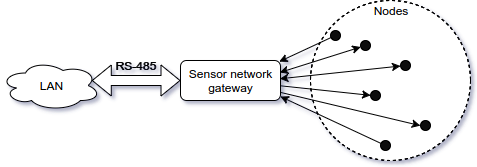
\includegraphics[width=1\textwidth]{01}
    \caption{Blokový diagram funkce gatewaye}
    \label{fig:block diagram of the system}
\end{figure}

Předpokládá se, že koncová zařízení jsou senzory nebo aktuátory napájeny z baterie, tudíž pro jejich dlouhodobou životnost je kladen důraz na nízkou spotřebu vybrané bezdrátové technologie.

Drátová síť RS485, přes kterou gateway komunikuje se PC masterem používá síťový protokol původně navržen pro přístupové systémy. 
Rošiřování vlastností tohoto protokolu by znamenalo mnoho komplikací, cílem je tedy implementace IoT tak, aniž by bylo nutné protokol rozšiřovat.


% todo: 
% - popiste infrastrukturu pristupovych systemu (obrazek a popis jednotlivych bloku), a jednak jejich vyuziti, zda se pouzivaji i na neco jineho - opet clanky, ten obr. 3.1 neni dostatecny pro clanek. Mam na mysli toto:
% https://www.elprocus.com/understanding-about-types-of-access-control-systems/
% https://en.wikipedia.org/wiki/Access_control#Access_control_system_topologies